\section{DayMOPS}
\label{linking}

Sufficiently bright moving objects which are observed by the LSST
telescope will generate DiaSource detections, stored in the LSST
DiaSource detection catalog.  The LSST DiaSource detection catalog
will also detections from a variety of other non-moving object
sources, including transient phenomena and artifacts of image
processing.

The LSST DayMOPS system is responsible for finding previously unknown
moving objects within the LSST DiaSource catalog.  Due to the large
number of detections expected, and the sometimes-unpredictable
behavior of asteroids with unknown orbits, a structured and
carefully-designed system is necessary to perform this searching and
discovery in a computationally efficient manner.






\subsection{Orbits}
Heliocentric orbits describe an orbit around the Sun.  Generally,
asteroids, planets and other solar system objects follow elliptical
paths, centered on the Sun.  These paths are described (in general
practice as well as the LSST Moving Objects catalog) with a Kepler
orbit, which describes an ellipse using six parameters. 

For purposes of DayMOPS and NightMOPS, we assume that a well-fitted
Kepler orbit should be sufficient to predict the location of an object
well into the future or past.  

\textbf{TBD: Illustration of a Kepler orbit - Wikipedia has a good one.}


\subsection{Orbit Determination and The Linking Problem}
Orbit determination refers to the problem of identifying an object's
orbit given a well-spaced set of detections of that object.  The
problem of orbit determination has been studied extensively \textbf{
  CITATIONS HERE }, and several software tools exist which can, given
a set of detections, identify an orbit which could have generated them
or identify that no such orbit could exist.We entrust that a suitable
outside tool will be chosen to handle this problem.

This leads to the non-trivial problem of correctly identifying that a
set of detections belonged to an unknown object and providing these
detections (and only those detections) to an orbit determination tool.
This is the \textbf{ linking problem}.  The majority of efforts in
the DayMOPS system have been directed at constraining the number of
linkages which are passed to the orbit determination tool, and at
methods for discovering those linkages quickly.

Fortunately, existing rules of thumb and approximations of asteroid
motion can be used both to predict possible linkages, and reject those
which are obviously untenable.

\subsubsection{Linear and Quadratic Models}
In order to discover and identify new objects, astronomers have
traditionally used sky-plane approximations to predict and model the
behavior of solar system objects for which a true orbit is not yet
known.  As a general rule of thumb, objects are said to move linearly
(with a more or less fixed velocity) in RA and Dec over the course of
a single night and quadratically (having velocity and some
acceleration) in RA and Dec over the course of a month.  These are, of
course, approximations, and linear and quadratic fits will inevitably
contain some error.

Given many detections which may or may not be attributable to one or
more asteroids, these approximations are used to help determine which
detections could plausibly be linked.  If several detections over the
course of a single night do not follow a roughly linear path, we trust
that they could not have been attributable to the same object; if
several detections over the course of a month do not follow a roughly
quadratic path, we will trust that they could not be attributable to
the same object.  By ignoring the obviously implausible linkages, we
significantly reduce the number of hypothetical linkages we must
investigate.

Of course, since these are merely approximations, it is almost
inevitable that some correct linkages will be rejected.  In
particular, some near-Earth-objects (NEOs) may exhibit sky-plane
behaviour not consistent with these rules of thumb.


\subsubsection{Higher-order Sky-Plane Models}
\textbf{TBD: Tim's methods go here - the assumed topocentric distance, topocentric correction, higher-order fits}


\subsection{The Linking Pipeline}
The linking pipeline is responsible for finding sets of detections
which may be attributable to the same moving object and sending them
to the Orbit Determination stage, which will either accept them as a
true linkage with an associated orbit or reject them as incorrectly
linked.  

To deal with the scale and complexity of discovering plausible
multi-night linkages for unknown objects, the DayMOPS system is
designed as a pipeline of several stages, building increasingly
sophisticated linkages at each step until multi-night linkages
suitable for orbit determination are discovered.  Specifically, we
move from individual detections to nightly, linear \textbf{tracklets},
to eventual multi-night \textbf{tracks} suitable for orbit
determination.  These tracks are filtered using a slightly more
sophisticated (but simpler than full orbit-space) model of asteroid
motion, to more quickly reject the (often numerous) mislinked tracks.

\textbf{TBD: Add an illustration of the various stages and a short piece of
introductory text.  Also perhaps useful: show one object's detections and its various states of linkage. (detections, tracklets, merged tracklets, track(s))}


Note that tracklets and tracks represent hypothetical linkages, many
of which may be correct.  A single detection may exist in several
tracklets and/or several tracks.  A given tracklet may be found in
multiple tracks.  Some detections may never be linked into any
tracklet; some tracklets will never be linked into any track.  The
DayMOPS system is built using methods and algorithms intended to
efficiently find plausible hypothetical linkages without wasting much
computational time or storage on finding unlikely linkages.



\subsection{Building Tracklets}

\textbf{ possible illustration: show Dec/time for two images, then tracklets in Dec/time}

\textbf{Tracklets} are linkages between DiaSource detections occuring
within the same night. By creating tracklets, DayMOPS can find
sky-plane position and velocity estimates for sets of detections which
may belong to the same solar system objects.  The use of tracklets
also simplifies the downstream work of track generation, which
attempts to find sets of detections with a good
position/velocity/acceleration fit on the sky-plane; since tracklets
have known position and velocity, the track generation phase needs
only to find those tracklets compatible within some acceleration
factor.

Correctly-linked tracklets from a given object are needed to generate
a good track for that object and eventually discover its orbit.
However, if these useful tracklets are too deeply buried among very
large numbers of other tracklets, then the job of tracklet linking
will become extremely slow and expensive.  Generally, these other,
unwanted tracklets are false tracklets (mislinkages between detections
not attributable to the same object), though in special conditions
large numbers of correctly-linked but redundant tracklets can cause
pain as well (this will discussed in \ref{collapseTracklets}).

In order to ensure that tracklet-generating images are acquired, it is
necessary to ensure that fields of the sky are visited two or more
times within an accepted time period each night. To constrain the
number of tracklets, we impose a maximum apparent velocity on the
tracklets, and also require that sky fields be revisited within a
fairly short time period ($\leq 90$ minutes is the current rule).
Raising the maximum velocity threshold enables one to find
faster-moving objects, and raising the maximum allowed revisit time
also enables one to generate tracklets in more fields of the sky;
however, increasing either of these thresholds also increases the
search space and can significantly increase the number of mislinked
tracklets, greatly increasing the cost downstream.




\subsubsection{The findTracklets Software}

The process of initial tracklet creation is accomplished by the
findTracklets software.  Later refinement of tracklets is accomplished
by collapseTracklets and additional filters.

\subsubsubsection{Algorithm} 

The findTracklets software is responsible for finding pairs of
detections which occur within a fixed time threshold, and have
apparent velocity below a given threshold.  For a given detection and
a set of image times, one can calculate the maximum distance an object
could have travelled at each time using the velocity limit.  To find
detections with which the query detection could be linked, one can
imagine searching a circular region in the later images based on this
distance.

\begin{figure}[ht!]
  \centering
    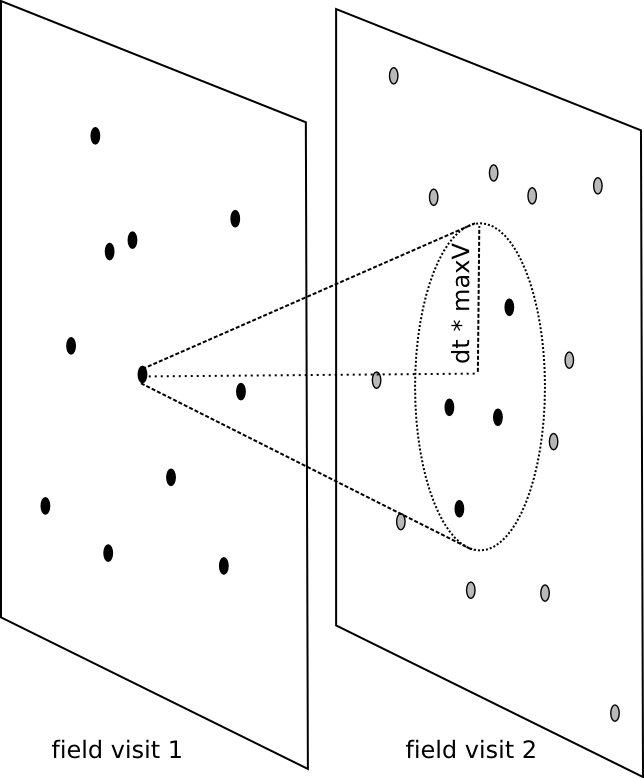
\includegraphics[width=6cm]{illustrations/findTracklets-onequery.png}
    \caption{ An example of searching for compatible second endpoints
      for a given detection.  The first detection and each of the
      second endpoints will be used to create a new tracklet.}
\label{findTrackletsIllustrated}
\end{figure}


Fortunately, this can be
accomplished in a fairly straightforward way through the use of
KD-Trees.  KD-Trees are a data structure which allows for quickly and
efficiently performing range searches on points in space
\citep{bentley_kdtrees}.  A KD-Tree-based method for building
tracklets was first contributed by Jeremy Kubica for his PhD thesis
\citep{kubica_thesis}.  For findTracklets, 2-Dimensional KD-Trees are
used, covering the space of (RA, Dec).  Given a detection and trees
containing detections from later images, we can use range searches to
quickly find nearby detections in those later images and use them for
the creation of tracklets.

\begin{figure}[ht!]
\begin{algorithmic}
\REQUIRE $I$ is a set of images, each of which has an associated exposure time and contains a set of detections
\STATE \COMMENT{Create a 2D KD-Tree for each image, holding detections from that image.}
\STATE $T \gets \{\}$
\FOR {$i \in I$}
  \STATE $t \gets$ Make2DTree$(i.detections)$
  \STATE $t.time \gets i.time$
  \STATE $T \gets T \cup \{t\}$
\ENDFOR
\STATE \COMMENT{Use these trees to discover the actual tracklets.}
\STATE $tracklets \gets \{\}$
\FOR {$t_1 \in T$}
  \STATE $later \gets \{t_i \in T : 0 < t_i.time - t_1.time < maxDt\}$
  \FOR{$d \in t_1.detections$}
     \FOR{$t_q \in later$}
 
       \STATE \COMMENT{Use time between images and max velocity to
         calculate the max travel distance}

        \STATE $dt \gets t_q.time - t_1.time$
        \STATE $dd \gets dt * maxV$
        \STATE \COMMENT{Use KD-Tree range search to find detections within max travel distance}
        \STATE $tracklets \gets tracklets \cup t_q.$rangeSearch($d.ra, d.dec, dd$)
     \ENDFOR
   \ENDFOR
\ENDFOR
\RETURN{$tracklets$}
\end{algorithmic}

\caption{Pseudo-code for the findTracklets algorithm.  2D (RA, Dec)
  trees are created for each image; for each detection, later trees
  are searched for nearby detections. }
 \label{findTrackletsAlgorithm}
\end{figure}


Note that because the sky is a sphere, notions of ``distance'' and
``velocity'' can become slightly confusing, especially near the poles.
Fortunately, both the KD-Tree library used and the findTracklets
software are sufficiently clever to use actual great-circle distance
and velocity for their queries, so that tracklets near the poles are
not missed.  The software should also be impervious to wrap-around
errors - objects which move between, say, $359.9 \degree$ in RA and
$.01 \degree$ in RA will be detected.  The Appendix \ref{kdTreeLib}
explains the KD-Tree library used in greater detail.  

\paragraph{Code and Usage}
Aside from the KD-Tree library, findTracklets is implemented by {\tt
  findTracklets.h}, {\tt findTracklets.cc } and a command-line
interface is provided by {\tt findTrackletsMain.cc}.  When calling the
function {\tt findTracklets()} programmatically (e.g. inside an LSST
Pipeline), use an instance of the {\tt findTrackletsConfig} to set the
values of all options (including max velocity and min/max time
threshold as well as others) and pass this to the {\tt
  findTracklets()} function.  See comments in {\tt findTracklets.h}
for documentation on the {\tt findTrackletsConfig} class.  Also see
\ref{largeData} for additional information on output methods.

The command-line {\tt findTracklets} program will take command-line
flags and use them to instantiate a {\tt findTrackletsConfig} which is
then used to call the actual {\tt findTracklets()} function.  Use {\tt
  \$findTracklets -h} for an overview of the options.






%%%%%%%%%%%%%%%%%%%%%%%%%%%%%%%%%%%%%%%%%%%%%%%%%%%%%%%%%%%%%%%%%%5
%% COLLAPSE TRACKLETS
%%%%%%%%%%%%%%%%%%%%%%%%%%%%%%%%%%%%%%%%%%%%%%%%%%%%%%%%%%%%%%%%%%5


\subsection{Improving and Filtering Tracklets} \label{collapseTracklets}
If a field of the sky gets multiple revisits, or more than two visits
within the time window, it is possible that findTracklets will find
more than one true tracklet associated with that object.  This can
generated needless downstream work, because the number of tracklets is
larger, and if the multiple true intra-nightly tracklets are never
linked together, then useful data (additional detections of the
object) can be lost, or may need to be pieced back together later.

In particular, in ``deep drilling'' operations, the telescope will
repeatedly image the same field of sky many times in a short period.
In these fields, the number of tracklets generated for an object will
grow like $O(n^2)$ where $n$ is the number of times the object is
seen, as each possible pair of detections will be linked.  This can
generate a huge number of tracklets, making later work exceptionally,
and needlessly, difficult.

The tracklet improvement and filtering stage attempts to remedy this
problem by joining together colinear 2-detection tracklets into
higher-cardinality (3 detections or more) tracklets.


\paragraph{Special Considerations}
There is a small risk that occasionally, a true 2-detection tracklet
be merged into a larger tracklet which is mislinked.  This is rare, as
it can only occur when a true tracklet is colinear with a mislinked
tracklet, but it is not strictly impossible.



\subsubsection{The collapseTracklets Software} 

The tracklet refinement and filtering stage actually consists of
several steps, which can be iterated as necessary.  The first and most
important stage is the collapseTracklets stage, which finds roughly
colinear tracklets and merges them.  

To accomplish this, a method similar to the Hough transform is used.
An intermediate time, $t_c$ is selected (we use the average time of
the first and last detections) and use the apparent linear motion of
the tracklets to project their location at $t_c$.  We then store these
projected (RA,Dec) locations and the angle/velocity of each tracklet.
At this point, colinear tracklets should have similar positions and
motion vectors, making them easy to find.  This is accomplished with a
series of range searches, which of course can be implemented with 4-D
(RA, Dec, angle, velocity) KD-Trees.  The full pseudo-code is
presented in Figure \ref{collapseTrackletsAlgorithm}.

\begin{figure}[ht!]
\begin{algorithmic}
  \REQUIRE $T$ is a set of intra-nightly tracklets, $D$ is the set of nightly detections from which $T$ was created, $range$ is a 4-tuple of tolerances for RA, Dec, angle and velocity.
  \STATE $t_c \gets midpoint(\{ d_{time} : d \in D \})$
  \FOR {$t \in T$}
    \STATE Calculate $t$'s predicted location at time $t_c$, its motion angle and velocity
  \ENDFOR
  \STATE \COMMENT{Create a 4D KD-Tree of the tracklets on their projected RA, Dec position and motion angle/velocity.}
  \STATE $tree \gets$ Make4DTree$(T)$
  \STATE $outTracklets = \{\}$
  \FOR {$t \in T,\ t$ has not already merged with another tracklet}
    \STATE \COMMENT{Find tracklets with projected location, motion similar to that of $t$}
     \STATE $outTracklets = outTracklets \cup tree.$rangeSearch$(t_{projected\ position}, t_{angle}, t_{velocity}, range)$
  \ENDFOR
  \RETURN{$outTracklets$}
\end{algorithmic}

\caption{Pseudo-code for the collapseTracklets algorithm. A 4-D KD-Tree over RA, Dec, angle, velocity is constructed using the projected locations and motion of the tracklets.  Tracklets which are similar in this 4-D space are roughly colinear, so they are merged and written to output}

\label{collapseTrackletsAlgorithm}

\end{figure}

Currently, collapseTracklets handles wrap-around, but otherwise treats
the sky as a flat (RA, Dec) plane when calculating the projected
positions of tracklets.  This is acceptable for tracklets close to the
ecliptic, but not sufficient closer to the poles.  This should be
fixed when possible.

Because the collapseTracklets algorithm does linking in
parameter-space, it is sometimes possible that the resulting tracklets
contain detections which are not quite colinear.  Also, some tracklets
may contain a superset of the detections present in other tracklets.
To address these, additional filtering stages are present.

\paragraph{Code and Usage}
The collapseTracklets algorithm is implemented in {\tt
  collapseTracklets.h} and {\tt collapseTracklets.cc}.  A command-line
interface is implemented in {\tt collapseTrackletsMain.cc}.  Run {\tt
  collapseTracklets -h} for usage hints.

Choosing an appropriate set of thresholds for collapseTracklets may be
difficult; with variable time between images, the amount of error on
velocity may differ from tracklet to tracklet.  Other factors come
into play as well; higher thresholds will lead to more correct
linkages as well as more incorrect linkages - which, as described in
the following section, can be ``undone'' later by purifyTracklets.  We
arrived at our current thresholds through simple trial and error.

\subsubsection{Tracklet Filtering Software}
The collapseTracklets algorithm attempts linking in parameter-space;
as a result, it is possible that tracklets which are not entirely
colinear may be merged.  This can be rectified using the
purifyTracklets algorithm, which removes detections from tracklets if
they are sufficiently off the best-fit line.  

Further, it is sometimes possible that a tracklet may link together a
set of detections already present in another, higher-cardinality
tracklet.  These ``subset tracklets'' are almost universally
unhelpful, and the removeSubsets algorithm may be used to efficiently
find and remove them from the active set of tracklets.


\begin{figure}[ht!]
\begin{algorithmic}
  \REQUIRE $T$ is a set of tracklets, $rmsMax$ is a maximum root-mean
  squared residual on the tracklet's best-fit function to its
  detections

  \FOR {$t \in T$}
    \STATE $rms = RMS(t)$
    \WHILE {$rms > maxRms, |t| > 2$} 
      \STATE remove the worst-fitting detection from $t$
      \STATE $rms = RMS(t)$
    \ENDWHILE
  \ENDFOR
  \RETURN{$outTracklets$}
\end{algorithmic}

\caption{In purifyTracklets, poorly-fitted detections are ``pruned''
  from tracklets. In certain degenerate cases, we may prune tracklets
  down to only two detections, in which case the pruning is
  abandoned.}

\label{purifyTrackletsAlgorithm}

\end{figure}


The subset removal algorithm can be used for tracklets as well as
tracks.  It is presented in \ref{subsetRemoval}.


\paragraph{Code and Usage}
We should really just kill off these silly sections and condense them
somewhere; everything has a foo.cc, foo.h and fooMain.h and a USAGE
string and a command-line calling convention and a library-style
calling convention, why repeat this everywhere?



\subsection{Building Tracks}

With tracklets already assembled, we should have many linkages
representing the position, location, and velocity of the various
objects observed, as well as ``false'', mislinked tracklets.  Making
use of the quadratic approximation of motion, valid for approximately
one month, we can move a sliding window of about 30 days over the
data, looking for tracklets which could be linked by some quadratic
acceleration factor.  As we find these linkages, we will also apply
some additional filters to avoid reporting those which are considered
too implausible (this will be described in \ref{trackFilters}.

Generally, the track generation phase is the most computationally
expensive task in DayMOPS processing; note that unlike other stages,
which consider only a night's-worth of data at a time, it must
consider tracklets from many nights and find linkages between them.
This task becomes far more difficult if the number of tracklets is
very large, either because the source data was very dense or the
thresholds were set very high, or because of poor refinement/merging
of intra-nightly tracklets.  Further, the relative looseness of the
quadratic approximation and the relative scarcity of data can make
track generation yet more difficult, as many plausible tracks may be
discovered.

Fortunately, a very clever algorithm for performing this track
discovery was presented by Kubica et al. (\citet{kubica_thesis},
\citet{Kubica:2005:MTA:1081870.1081889}).  In essence, the idea behind
the algorithm is to build per-image 4D-Trees of (RA position, Dec
position, RA velocity, Dec velocity), and use these to hold the
tracklets, indexed by position/velocity.  We then imagine the KD-Trees
as hierarchical bounding boxes, and consider sets of bounding boxes,
calculating whether they could be linked by some acceleration factor
less than our maximum acceleration threshold.  If the boxes could be
linked, then a track may exist within their contents and we continue
searching bounding boxes lower in the tree hierarchy; if not, we know
that no track of interest to us could pass through the boxes and we
can abandon searching immediately.  By using the hierarchical
structure of the KD-Trees, we can avoid searching in large areas of
tracklet-space where no track could ever exist, greatly reducing our
workload.


\subsubsection{Search Pruning}

A KD-Tree node can be thought of as representing a bounding box in (RA
position, Dec position, RA velocity, Dec velocity) space.  When
examining a pair of KD-Tree nodes, we wish to answer the question:
could a tracklet from the first node ever enter the second, within a
fixed min/max acceleration? Considering RA and Dec seperately, we can
calculate the minimum and maximum accelerations needed for a point in
the first bounding box to reach the second.  If the acceleration is
too high or low (say, $>.02 deg/day^2$ or $<-.02 deg/day^2$, then we
know that no track of interest to us could pass from the first node to
the second.

When we consider two KD-Tree nodes, $Node1$ and $Node2$, each
encompassing a region of position/velocity space, we can calculate the
possible range of accelerations in RA and Dec which could connect
points in $Node1$ to points in $Node2$, through formulae derived from
$p = p0 + vt + frac{1}{2}at^2$.  Further, since we are only interested
in tracks with a given velocity range, we also have a user-specified
minimum/maximum acceleration range; since the bounding boxes/KD-Tree
nodes are hierarchical, we can constrain the allowable acceleration
bounds by the bounds of the parent boxes of $Node1$ and $Node2$.  We
calculate the acceleration bounds using the following equation, with
the variables $parentMinAcc$ and $parentMaxAcc$ representing the
inherited min/max bounds from the parent or, in the case that the
nodes have no parents, the user-specified min/max accelerations:

\begin{equation}
maxAcc = \min \left(\begin{array}{ccc} & \displaystyle parentMaxAcc, \\
& \displaystyle \frac{Node2.maxV - Node1.minV}{dt} \\
& \displaystyle \frac{2}{dt^2} \bigg(Node2.maxP_0 - Node1.minP_0 - Node1.minV \times dt \bigg) \\
& \displaystyle \frac{2}{dt^2} \bigg(Node1.maxP_0 - Node2.minP_0 + Node2.maxV \times dt \bigg) \end{array}\right)
\end{equation}

\begin{equation}
minAcc  = \max \left(\begin{array}{ccc} & parentMinAcc,\\
& \displaystyle \frac{Node2.minV - Node1.maxV}{dt},\\
& \displaystyle \frac{2}{dt^2} \bigg( Node2.minP_0 - Node1.maxP_0 - \displaystyle Node1.maxV \times dt\bigg), \\
& \displaystyle \frac{2}{dt^2} \bigg(Node1.minP_0 - Node2.maxP_0 + Node2.minV \times dt\bigg) \end{array} \right)
\end{equation}

Note that this approach simplifies the problem by treating the sky as
a Cartesian plane, which will be problematic near the poles.  However,
the above calculation appears to be the ``hot spot'' of the
linkTracklets algorithm and accounts for most of the computation time,
and so simplifying to reduce floating point costs affords far better
performance.

In the code, this calculation is performed by the function {\tt
  updateAccBoundsReturnValidity} in {\tt linkTracklets.cc}.

\subsubsection{Recursive Tree-walk Using Pruning}

support trees here?  maybe algorithm with and without support trees?

psuedocode basically like Kubica's, note location in code

\subsubsection{Terminal Processing - Actual Track Generation}

give a forward-reference to track filtering methods, note location in code

\subsubsection{Overall Algorithm}

Note location in code

\subsubsection{Subtle Quirks}

Astrometric error on detections will affect both the position and
velocities of true tracklets.  As a result, bounding boxes must be
extended to encompass not just the tracklets which they hold, but the
surrounding error bars.  As a result, tracklet bounding boxes (KD-Tree
nodes) are extended using the following equation, where $dt$ is the
\textit{shortest} time span of any tracklet in the bounding box:

\begin{eqnarray}
minP_0 = P_0 - astrom\_err \\
maxP_0 = P_0 + astrom\_err \\
minV = (deltaP - 2\times astrom\_err)/dt  \\
maxV = (deltaP + 2\times astrom\_err /dt
\end{eqnarray}






Each tracklet represents a possible object on a given night, and the
position and velocity of that object.  The track generation phase uses
these tracklets to find tracks, which present a hypothetical object
with

Over the course of roughly one month, solar system objects tend to
follow a roughly quadratic path on the sky-plane
\citep{kubica_thesis}.  The track generation phase of DayMOPS will
attempt to find sets of tracklets (which have position and velocity
estimates) which were observed within one month of each other and are
compatible within some acceleration range.  Tracks which are
suitable for generating a reasonable orbital fit are sent to the Orbit
Determination phase.

The methods used for tracklet-to-tracklet linking are described in
\citet{kubica_thesis} and \citet{Kubica:2005:MTA:1081870.1081889}.
The methods described attempt to efficiently find sets of tracklets
which are \textit{compatible} in the sense that they could be joined
to form a track: that is, tracklets which span multiple nights and
have positions and velocities which are consistent with a fixed
acceleration.  

To perform this work efficiently, these methods use four-dimensional
KD-Trees over \textit{tracklet-space}, or (RA position, Dec position,
RA velocity, Dec velocity). One tree is created per image, and holds
each tracklet which has its first detection in that image.  A
multi-tree walk is performed using a clever algorithm, efficiently
discovering all regions of tracklet-space which could contain sets of
tracklets that are compatible, while avoiding visits to tracklet-space
regions which are not compatible and could not generate a track.  This
is performed recursively until leaf nodes of the KD-Trees are reached.

% illustration from Kubica?

When the algorithm encounters a set of leaf nodes in the KD-Trees, it
attempts to build a track using the detections held in the tracklets
at the leaf nodes.  A quadratic fit, or a higher-order fit if
possible, to the detections will be attempted.  Then a quality-of-fit
assessment is used to determine whether the track is considered
sufficiently well-fitted to pass downstream to the Orbit
Determination.  Investigation into ideal higher-order fits and
quality-of-fit metrics is ongoing, but as of this writing a filter on
minimum chi-squared probability appears to be the best option.

\subsubsection{The linkTracklets Software}
Cover the code, its status, what routines do what in the psuedocode,
etc.  Also cover hotspots, sensitive areas, and parameters which have
big impacts on behavior here.


\subsection{Filtering of Tracks}
\label{trackFilters}
Some more information on implementation of Tim's fitting and
chi-squared filter and the software. Stats on ground-truth fitting,
possible needs for improvements.


\subsection{Notes on the Linking Software}

\subsubsection{Accomodations for Large Data Sets}
\label{largeData}
Over the course of our experiments, we discovered that under some
circumstances, tools may return some very large data sets - larger
than the memory available on our development machines.  Though RAM
sizes may grow over time, it is likely that DayMOPS users will
continue to experiment with increasingly dense noise or loose limits,
resulting in increasingly large numbers of tracklets or tracks.

To help deal with this problem, the {\tt  findTracklets} and
{\tt linkTracklets} functions can be configured to output their results
in various ways; they can be configured either to store their results
in memory and return them (much like a normal function call) or to
return nothing and write results directly to file.  If the user is
confident that the data set to be returned will fit in memory, the
former is more elegant, but for our experiments we always write to
file first, in case the number of tracklets or tracks discovered is
large.

The {\tt findTracklets} and {\tt linkTracklets} functions each take as
an argument an object of type {\tt findTrackletsConfig} or
{\tt linkTrackletsConfig}; each type has a public member variable
called {\tt outputMethod} which can be set.  {\tt findTracklets.h} and
{\tt linkTracklets.h} each contain enum types which can be used to set
these flags.

Dealing with larger-than-memory data sets as input to our software
tools is a more significant problem.  We generally assume that the
number of input detections will fit in memory, and that KD-Trees of
these detections will also fit in memory.  This has always been the
case, and fortunately it is easy to predict whether a set of
detections will fit in memory or not.  However, the number of
tracklets or tracks may, depending on the data and configuration of
the software, grow to be quite large, and is not trivially
predictable.  For software which uses tracklets or tracks as its input
data and operates on them in bulk (including {\tt collapseTracklets},
{\tt removeSubsets}, and {\tt linkTracklets}), this may be problematic;
see section \ref{parallelization} for more information on this
problem.




\subsection{Orbit Fitting}
\label{orbitFitting}

Orbit fitting can be accomplished using either traditional geometric
methods, where an ellipse or parabola consistent with movement in the
gravitational field of the sun is fit to the set of detections, or
with statistical ranging, where a wide range of potential orbits are
evaluated against the set of detections to search for those with
the lowest residuals. Traditional methods are typically much speedier,
and are available to LSST through the OrbFit software from Milani
\citep{Milani2006}. Statistical ranging methods are more accurate in
exploring the full range of orbital uncertainties for each object,
which can be particularly important for objects observed near 60--90
degrees from the Sun where NEO and MBA exhibit similar apparent
motions, and are available in the OpenOrb software from Granvik
\citep{OpenOrb2009}.

In general, orbit fitting is split into two conceptual pieces - an
``initial orbit determination'' stage, where approximate orbits are
calculated, and a ``differential correction'' stage, where
perturbations on the initial orbit are evaluated to find the best fit
and uncertainty. With six observations on three different nights, most
real moving objects will pass both initial orbit determination and
differential correction with an orbit accurate enough to generate
predicted positions with uncertainties of less than a few arcminutes
for the next few months \citep{basicSolarSystem}.





\subsection{Sky-Plane Motion Limits Imposed by Sky-Plane Linking Methods}

Practical considerations necessitate that we set upper bounds on
tracklet velocity and track acceleration in order to restrict the
number of potential mislinkages. Existing methods attempt to find all
tracklets or tracks within specified velocity and acceleration limits;
as velocity and acceleration limits are raised, the number of
tracklets and tracks can grow quickly.  As a result, the choice of
velocity and acceleration limits is important, as it significantly
impacts the objects found as well as the cost of running the software.

Generally, all types of solar system objects except for the fastest of
near-earth asteroids tend to have reasonably low sky-plane velocity
and acceleration. It is expected that the fastest-moving objects will
leave visible trails in images; these may be used to isolate
detections which could be attributable to fast-movers and restrict the
potential search space for linking these detections.  See section
\ref{neosTrailing} for more information on future plans for
approaching this problem.  

